

\documentclass[a4paper]{article}

\usepackage{amsmath}
\usepackage{hyperref}
\usepackage{biblatex}
\usepackage{enumerate}
\usepackage{graphicx}
\usepackage{stmaryrd}
\usepackage[dvipsnames]{xcolor}
\usepackage{listings}
\usepackage{caption}
\usepackage{subcaption}
\usepackage{booktabs}


\addbibresource{refs.bib}

\begin{document}

\author{Ola Bratt \\
  \href{mailto:ola.bratt@gmail.com}{ola.bratt@gmail.com}
  \and
  Patrick Attimont \\
  \href{patrickattimont@gmail.com}{patrickattimont@gmail.com}
}

\title{DAT565/DIT407 Assignment 3}
\date{2024-02-xx}

\maketitle

This paper is addressing the assignment 3 study queries within the \emph{Introduction to Data Science \& AI} course, DIT407 at 
the University of Gothenburg and DAT565 at Chalmers. The main source of information for this project
is derived from the lectures and Skiena~\cite{Skiena:2024}. 

\section*{Problem 1: Spam and Ham}

\section*{Problem 2: Preprocessing}

\section*{Problem 3: Easy Ham}

\begin{table}
  \begin{center}
  \begin{tabular}{ l|l|l|l|l }
    \hline
    \text{Model} & \text{accuracy} & \text{precision} & \text{recall} & \text{F1 score}\\
    \hline
    \text{Multinomial Naive Bayes} & 0.9852700490998363 & 0.9844357976653697 & 0.9980276134122288 & 0.991185112634672 \\
    \text{Bernoulli Naive Bayes} & 0.9230769230769231 & 0.9181818181818182 & 0.9960552268244576 & 0.9555345316934721 \\
  \end{tabular}
\end{center}
\caption{Precision and accuracy for Easy Ham and Spam}
  \label{tabular:easy_summary}
\end{table}


\begin{figure}
  \centering
  \begin{subfigure}[a]{\textwidth}
      \centering
      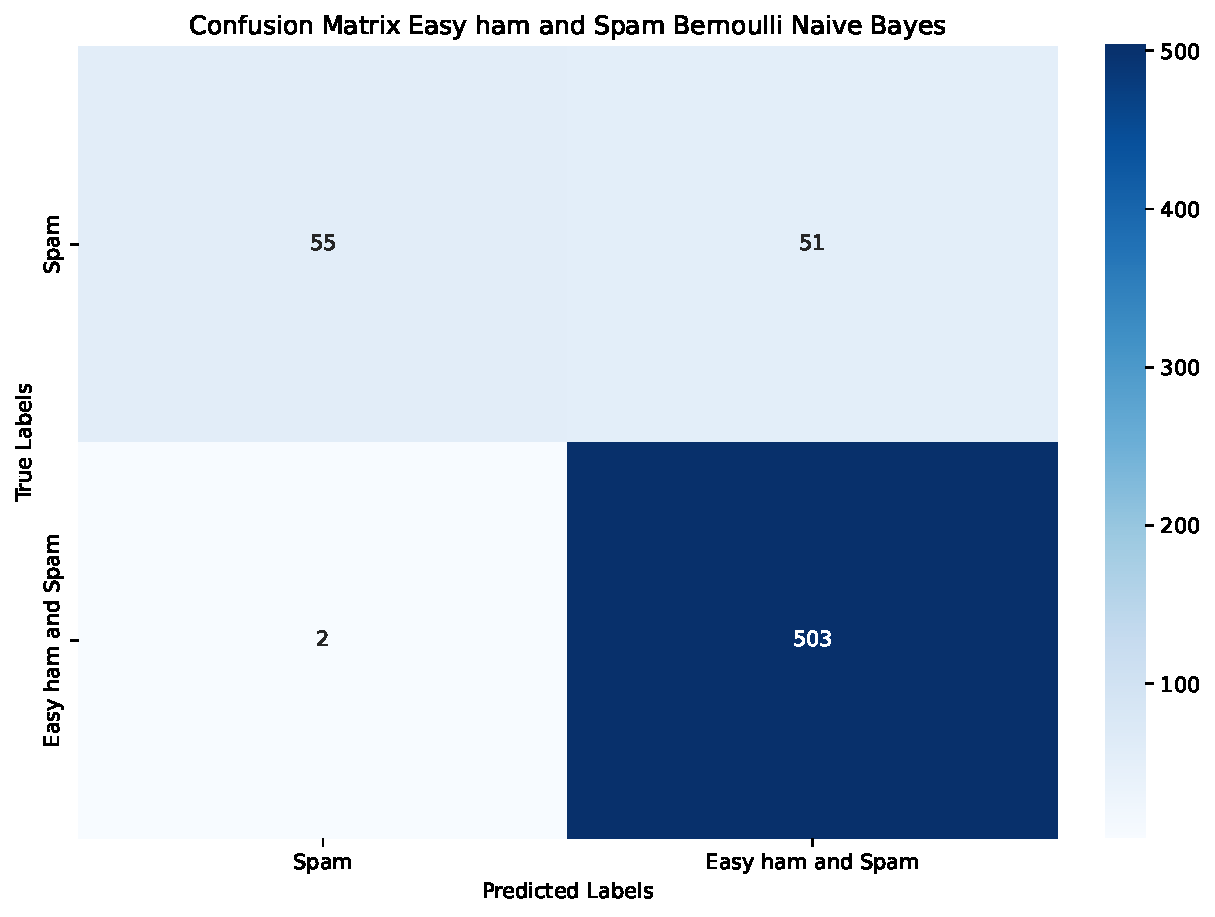
\includegraphics[width=\textwidth]{easy_ham_and_spam_bernoulli_naive_bayes_confusion_matrix.pdf}
      \caption{Easy ham vs spam, Bernoulli Naive Bayes}
      \label{fig:easy_ham_and_spam_bernoulli_naive_bayes_confusion_matrix}
  \end{subfigure}
  \vfill
  \begin{subfigure}[b]{\textwidth}
      \centering
      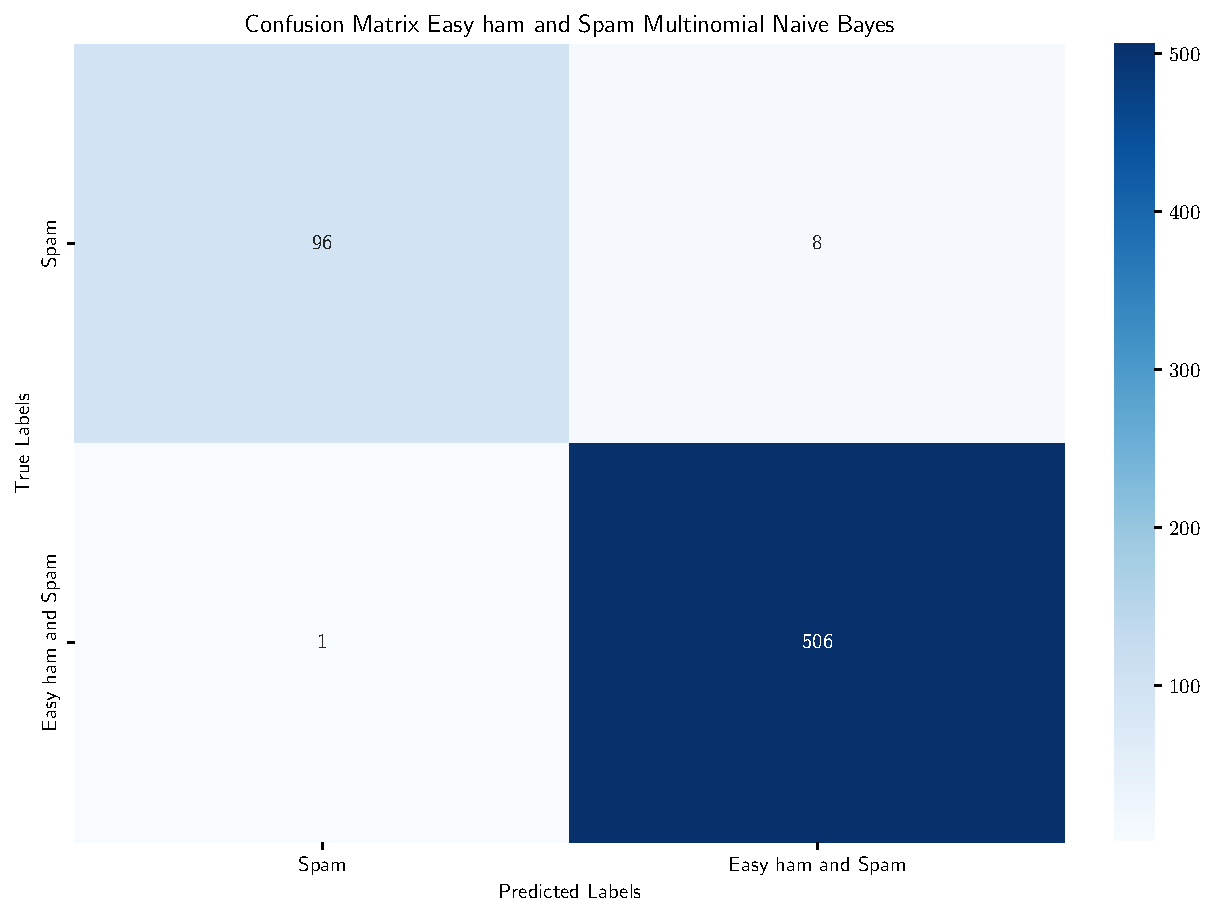
\includegraphics[width=\textwidth]{easy_ham_and_spam_multinomial_naive_bayes_confusion_matrix.pdf}
      \caption{Easy ham vs spam, Multinomial Naive Bayes}
      \label{fig:easy_ham_and_spam_multinomial_naive_bayes_confusion_matrix}
  \end{subfigure}
  \caption{Confusion matrixes of easy ham and spam}
  \label{fig:easy_ham_and_spam_confusion_matrix}
\end{figure}

\newpage
\section*{Problem 3: Hard Ham}


\begin{table}
  \begin{center}
  \begin{tabular}{l|l|l|l|l}
    \hline
    \text{Model} & \text{accuracy} & \text{precision} & \text{recall} & \text{F1 score}\\
    \hline
    \text{Multinomial Naive Bayes} & 0.9470198675496688 & 0.9555555555555556 & 0.8775510204081632 & 0.9148936170212767 \\
    \text{Bernoulli Naive Bayes} & 0.9337748344370861 & 0.975609756097561 & 0.8163265306122449 & 0.888888888888889 \\
  \end{tabular}
\end{center}
\caption{Precision and accuracy for Hard Ham and Spam}
  \label{tabular:hard_summary}
\end{table}

\begin{figure}
  \centering
  \begin{subfigure}[a]{\textwidth}
      \centering
      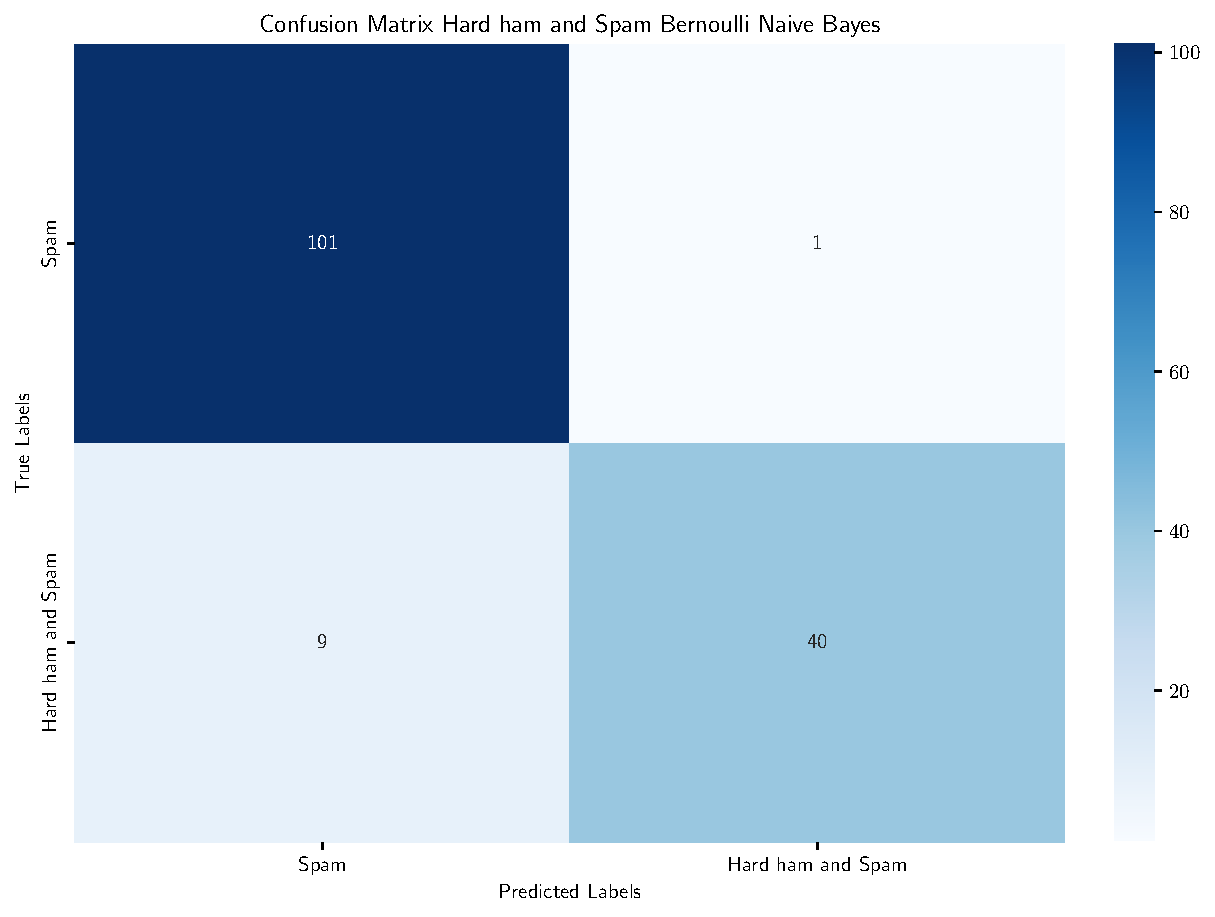
\includegraphics[width=\textwidth]{hard_ham_and_spam_bernoulli_naive_bayes_confusion_matrix.pdf}
      \caption{Hard ham vs spam, Bernoulli Naive Bayes}
      \label{fig:hard_ham_and_spam_bernoulli_naive_bayes_confusion_matrix}
  \end{subfigure}
  \vfill
  \begin{subfigure}[b]{\textwidth}
      \centering
      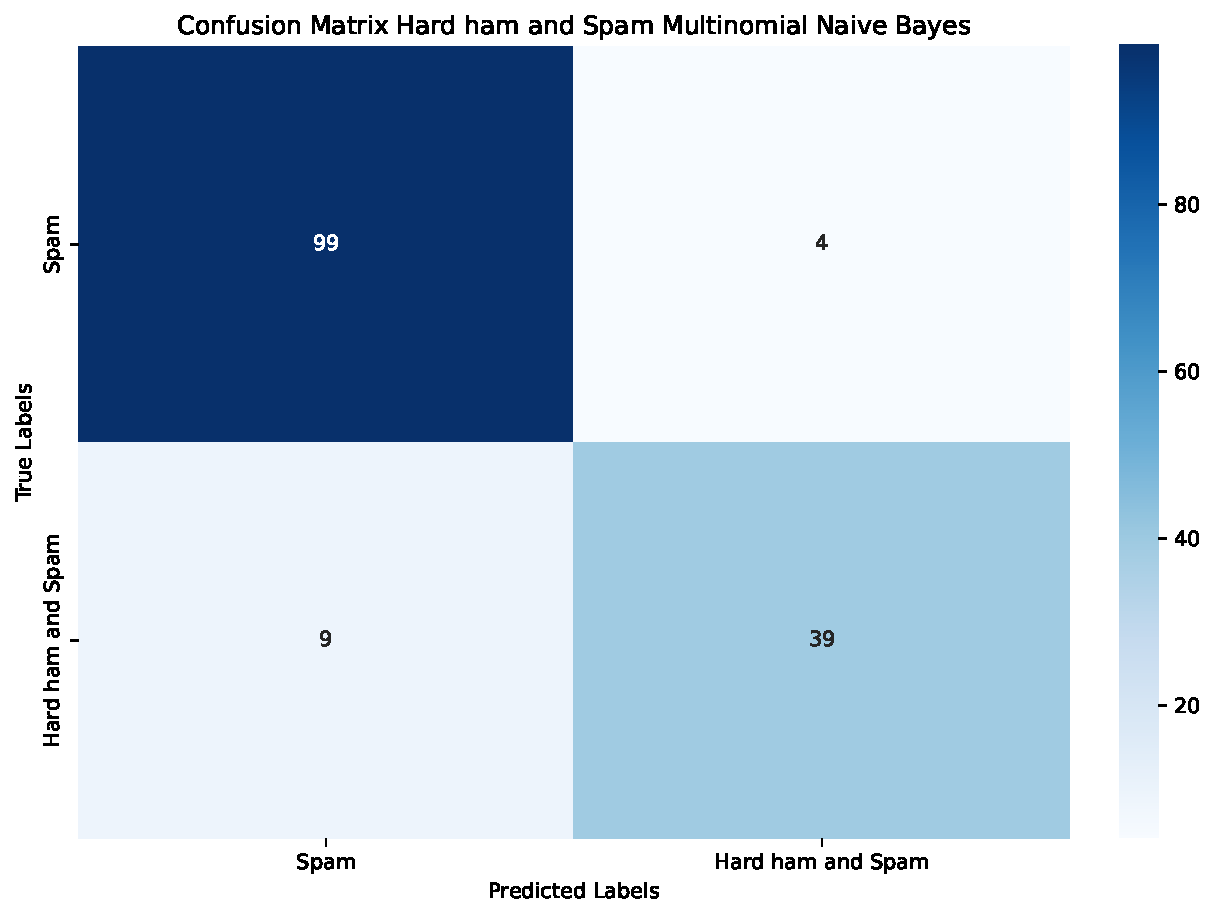
\includegraphics[width=\textwidth]{hard_ham_and_spam_multinomial_naive_bayes_confusion_matrix.pdf}
      \caption{Hard ham vs spam, Multinomial Naive Bayes}
      \label{fig:hard_ham_and_spam_multinomial_naive_bayes_confusion_matrix}
  \end{subfigure}
  \caption{Confusion matrixes of hard ham and spam}
  \label{fig:hard_ham_and_spam_confusion_matrix}
\end{figure}

\newpage





\printbibliography

\section*{Appendix: Source Code}

\lstset{
  language=Python,
  basicstyle=\ttfamily,
  commentstyle=\color{OliveGreen},
  keywordstyle=\bfseries\color{Magenta},
  stringstyle=\color{YellowOrange},
  numbers=left,
  basicstyle=\footnotesize,
  breaklines=true,
  postbreak=\mbox{\textcolor{red}{$\hookrightarrow$}\space}
}


%\lstinputlisting{ola/assignment3.py}

\end{document}
